\section{EXPERIMENTAL RESULTS}\label{sec:4experiment}
In this section, we discuss the experiment methodology and detail the evaluation results.



\subsection{Evaluation Results}
We focus on the detection accuracy about five events, that are body posture, the body rollover, the hand position and  the acoustic events.
%, the classification of micro body movement

\subsubsection{Performance of body posture calssification}
To test the detection accuracy of different body postures, we use the data of User 1 to train the classifier. Then this classifier is used for other nine persons. Fig. \ref{fig:posture} plots the performance across different users. We observe that the posture detection accuracy is consistently high across all users, and it does not show major variations across users. However, we find that the supine posture and prone posture have lower accuracy comparing the other two lateral postures, that are 92\% and 85\%, respectively. This is because the hand positions under the prone posture and supine posture are similar, and the direction sensor suffers high sensitivity.

\begin{figure}[!thbp]
 \centering
 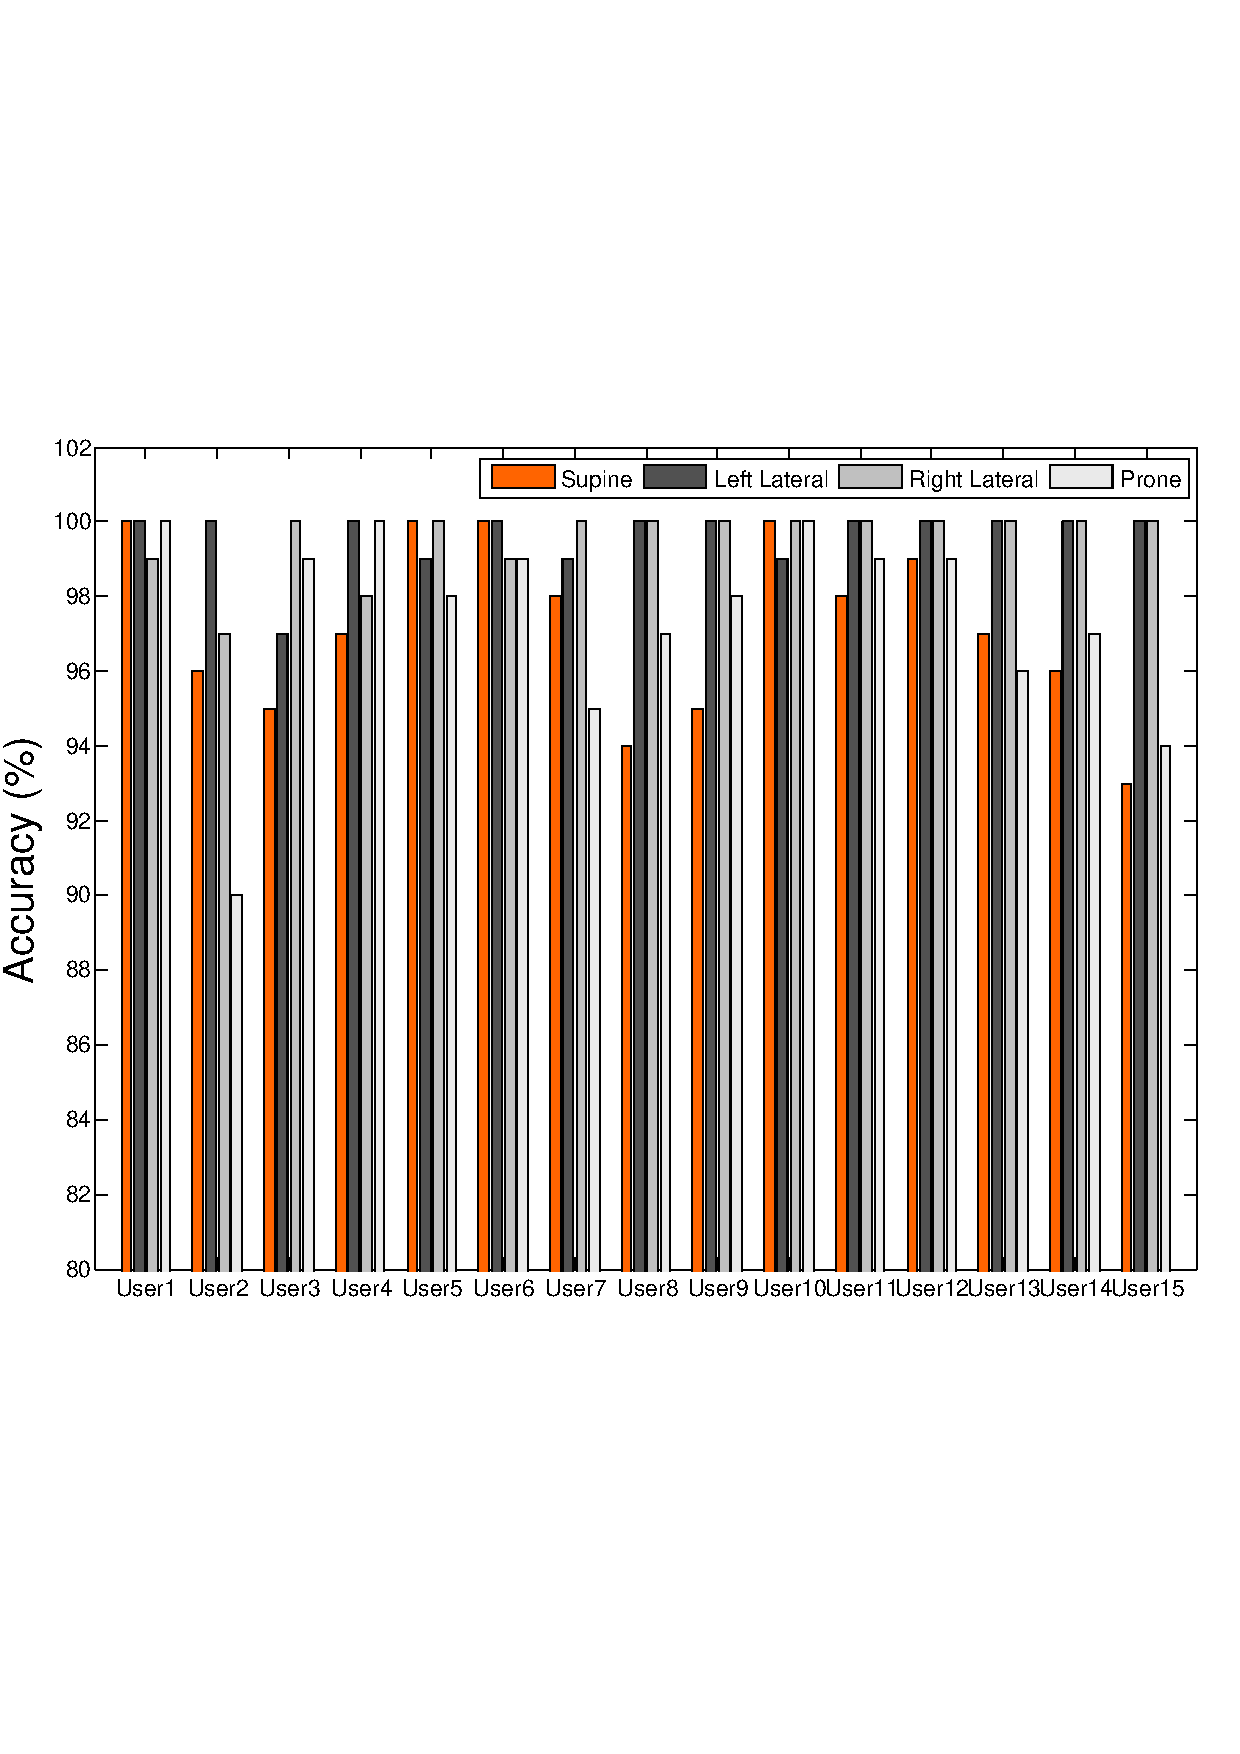
\includegraphics[width=0.77\linewidth]{Figures/posture_zhu.pdf}
 \caption{Detection accuracy of body postures.}\label{fig:posture_zhu}
 \end{figure}

Then to test the overall body detection performance, we calculate the detection precision and recall across all postures. The result is shown in Table \ref{tab:posture}. The values in  blocks are the corresponding numbers of the four types of sleep postures in our testing data. As we can see, the total amount of the prone posture is less than the number of other postures. It suggests that most people are not accustomed to sleep in the prone posture, because it is neither healthy nor comfortable. All in all, Table \ref{tab:posture} shows the outstanding detection performance.

\begin{table}[!thbp]
  \centering
  \tabcolsep1pt
  %\arrayrulewidth1pt
  \renewcommand\arraystretch{0.277}
  \caption{The confusion matrix of body posture classification.}\label{tab:posture}
  \noindent\makebox{%
\begin{tabularx}{1\textwidth}{ c | c | c | c | c | c | c}
   \cline{1-7}
   &\multicolumn{1}{ c|}{ }
   & \multicolumn{4}{ c|}{ }\\
   \multirow{2}*{}
&\multicolumn{1}{c|}{\multirow{2}*{{Result}}}
&\multicolumn{4}{c|}{{Prediction}}
& \multirow{4}*{{Recall}} \\
    %&\multicolumn{5}{ c |}{\textbf{\small Prediction}} \\
   % & \multicolumn{5}{ c |}{ } \\
    \cline{3-6}
    & & & & & \\
    \multicolumn{1}{c|}{{}}
    &  \multicolumn{1}{c|}{{}}
    &  \multicolumn{1}{c|}{{Supine}}
    &  \multicolumn{1}{c|}{{Left Lateral}}
    &  \multicolumn{1}{c|}{{Right Lateral}}
    &  \multicolumn{1}{c|}{{Prone}}   \\
    & & & & & \\
     \cline{1-7}
    & & & & & \\
    \multirow{5}{*}{\begin{sideways}{{Groundtruth}}\end{sideways}}
    &   {Supine}   & {\bf{{117}}}    &   $0$      &   $0$      &   $3$    &   {97.4\%}\\
    & & & & & \\
    \cline{2-7}
    & & & & & \\
   &   {Left Lateral}   &   $0$      &   {\bf{{123}}}     &   $0$      &   $0$   &   {100\%} \\
    & & & & & \\
     \cline{2-7}
    & & & & & \\
    &   {Right Lateral}   &   $0$      &   $0$      &  {\bf{{146}}}      &   $0$  &   {100\%}  \\
    & & & & & \\
     \cline{2-7}
    & & & & & \\
    &   {Prone}   &   $6$      &   $0$      &   $0$      &   {\bf{{64}}}   &   {91.4\%} \\
    & & & & & \\
    \cline{1-7}
    & & & & & \\
    &   {Precision}    &   {95.1\%}   &   {100\%}   &   {100\%}   &   {95.5\%}    \\
    & & & & & \\
    \cline{1-7}
   \end{tabularx}}
\end{table}


\subsubsection{Performance of body rollover counting}
To verify the efficiency of body rollover detection algorithm, we  compare the number of body rollover detected by {\systemname} with the groundtruth number recorded by camera. The detection performance is showed in Table \ref{tab:rollver}. For 10 users, the average detection accuracies are all very high, and the least one is still 87\%. Thus our system can accurately distinguish the large hand movement from the body rollover in bed.

\begin{table}[!thbp]
  %\centering  % ������
  \tabcolsep 1pt
  %\arrayrulewidth1pt
  \caption{Detection accuracy of  body rollover.}\label{tab:rollver}
   \renewcommand\arraystretch{1.3}{\multirowsetup}{\centering}
        \begin{tabular}{c|cccccccccc}
        \cline{1-11}
         { User}    & 1& 2  & 3& 4& 5& 6& 7& 8& 9& 10\\
                \cline{1-11}
               { Groundtruth}  &35&34&28&30&25&47&30&39 &43& 36  \\
                \cline{1-11}
                 { Accuracy} &91\%& 94\% &90\%&93\%&96\%&94\%&87\%&90\% &93\% &97\%  \\
        \cline{1-11}
 \end{tabular}
\end{table}


 \subsubsection{Performance of hand position recognition}
%To test the identification performance of hand position, we investigate the breathing detection accuracy first. Fig. \ref{} shows the breathing identification accuracies of hand on the chest or abdomen across 10 users. It indicates that our system can detect the breathing at most time. Note that when we detect the breathing, the hand position is unknown for us.

%After the breathing detection stage,

To test the identification performance of different hand positions, {\systemname} uses the data of User 1 to train the classifier. The classifier is used to detect the hand moving trajectory, then the hand position which is on the chest or abdomen can be identified.  Fig. \ref{fig:hand_zhu} illustrates the accuracy of hand position across 10 people. With just one set of training data, the accuracies for different users are all higher than 87\%.  Therefore, our system can achieve a satisfied identification accuracy for different hand positions.

\begin{figure}
 \centering
 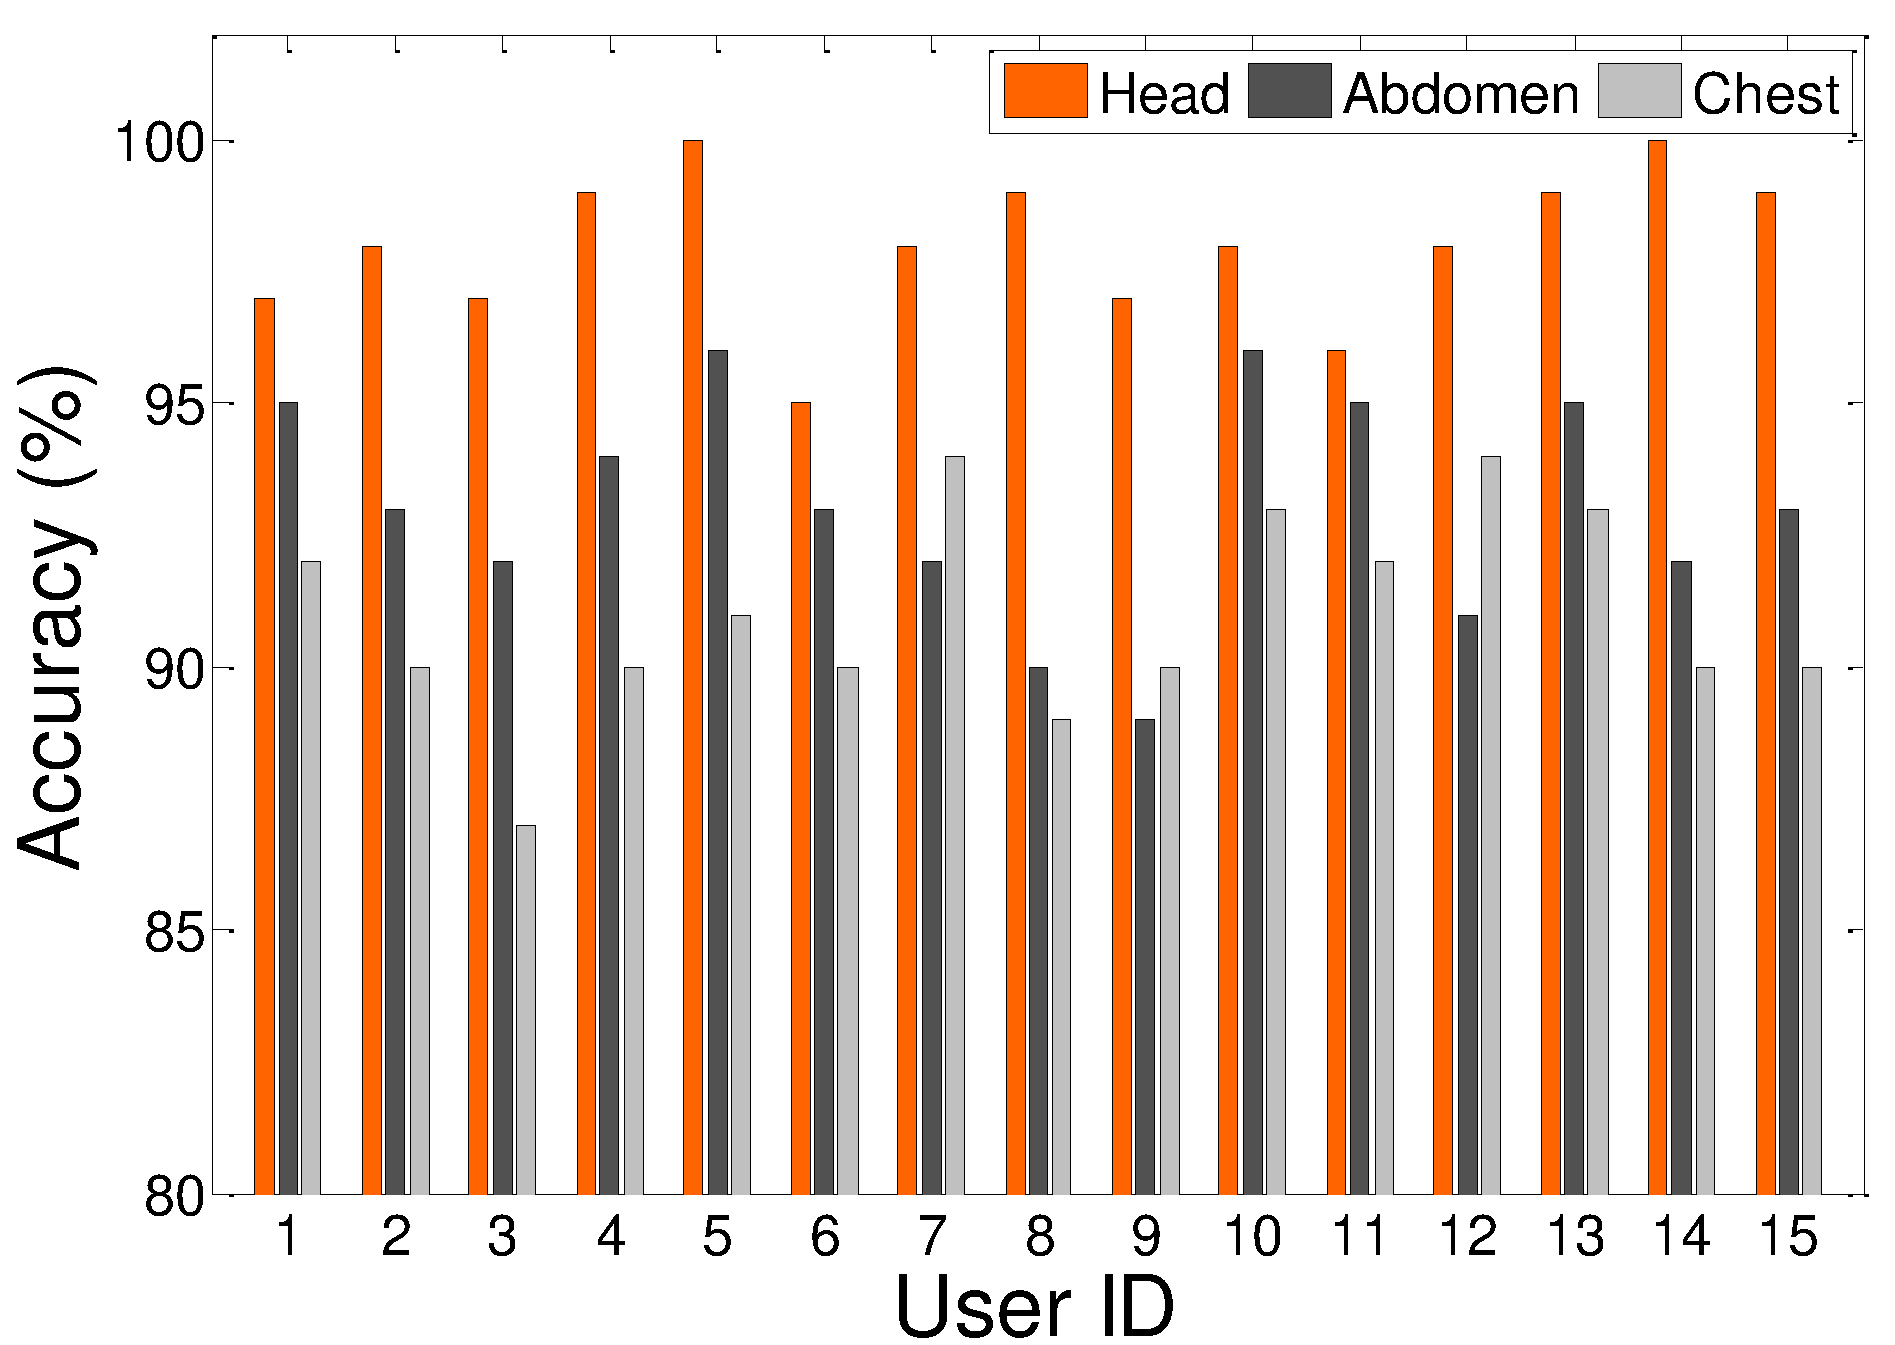
\includegraphics[width=0.77\linewidth]{Figures/handposition_zhu.pdf}
 \caption{Identification accuracy of hand positions}\label{fig:hand_zhu}
\end{figure}




%\subsubsection{Micro body movement}






 \subsubsection{Performance of acoustic events detection}
To study the detection accuracies of different acoustic events, we compare the groundtruth recorded by the camera with the detected results by our system. The parameters used in the detection algorithms are trained by User 1. Table \ref{tab:sound} shows the results across 10 users. We can see that the accuracy for snore event is 94.7\%, which is relative lower with regard to other three events. The reason is that different user's snore pattern are different,  the pre-defined parameters used in the system does not include all possible patterns of snore events. To improve the detection accuracy, we can train particular parameters for different users.

\begin{table}[!thbp]
 \tabcolsep1pt
  \centering  % ������
  \renewcommand\arraystretch{0.3}
  \caption{The confusion matrix of acoustic events detection.}\label{tab:sound}
\begin{tabular}{c| c | c | c | c | c | c}
   \hline
   &\multicolumn{1}{ c|}{ }
   & \multicolumn{4}{ c|}{ }\\
   \multirow{2}*{}
&\multicolumn{1}{c|}{\multirow{2}*{{ Result}}}
&\multicolumn{4}{c|}{{ Prediction}}
& \multirow{4}*{{ Recall}} \\
    %&\multicolumn{5}{ c |}{\textbf{\small Prediction}} \\
   % & \multicolumn{5}{ c |}{ } \\
    \cline{3-6}
    & & & & & \\
    \multicolumn{1}{c|}{{}}
    &  \multicolumn{1}{c|}{{}}
    &  \multicolumn{1}{c|}{{ Snore}}
    &  \multicolumn{1}{c|}{{ Cough}}
    &  \multicolumn{1}{c|}{{ Somniloquy}}
    &  \multicolumn{1}{c|}{{ Other}}   \\
    & & & & & \\
     \cline{1-7}
    & & & & & \\
    \multirow{5}{*}{\begin{sideways}{{ Groundtruth}}\end{sideways}}
    &   { Snore}   & {\bf{{18}}}    &   $0$      &   $0$      &   $3$    &   {85.7\%}\\
    & & & & & \\
    \cline{2-7}
    & & & & & \\
   &   { Cough}   &   $1$      &   {\bf{{34}}}     &   $0$      &   $1$   &   {94.4\%} \\
    & & & & & \\
     \cline{2-7}
    & & & & & \\
    &   { Somniloquy}   &   $0$      &   $1$      &  {\bf{{8}}}      &   $1$  &   {80\%}  \\
    & & & & & \\
     \cline{2-7}
    & & & & & \\
    &   { Other}   &   $0$      &   $0$      &   $0$      &   {\bf{{160}}}   &   {100\%} \\
    & & & & & \\
    \hline
    & & & & & \\
    &   { Precision}      &   {94.7\%}   &   {97.1\%}   &   {100\%}   &   {97.0\%}    \\
    & & & & & \\
    \hline
   \end{tabular}
\end{table}


\subsection{Overall performance}

In order to measure the sleep stage performance of {\systemname}, the volunteers are asked to wear Zeo \cite{zeo} during their sleep. Then we compare the results of sleep stage detection from Zeo and those of our system.  We regard the detection results of Zeo as the groundtruth. The average values of precision and recall are shown in  Table \ref{tab:sleep stage}. From this table, we can see that although {\systemname} may often make misjudgement between light sleep stage and REM, the overall detection performance of Sleep Hunter is satisfying.

\begin{table}[!thbp]
 \tabcolsep1pt
  \centering  % ������
  \renewcommand\arraystretch{0.4}
  \caption{ Performance of sleep stage detection.}\label{tab:sleep stage}
\begin{tabular}{c| c | c | c | c | c}
   \hline
   &\multicolumn{1}{ c|}{ }
   & \multicolumn{3}{ c|}{ }\\
   \multirow{2}*{}
&\multicolumn{1}{c|}{\multirow{2}*{{ Result}}}
&\multicolumn{3}{c|}{{ Prediction}}
& \multirow{3}*{{ Recall}} \\
    %&\multicolumn{5}{ c |}{\textbf{\small Prediction}} \\
   % & \multicolumn{5}{ c |}{ } \\
    \cline{3-5}
    & & & & & \\
    \multicolumn{1}{c|}{{}}
    &  \multicolumn{1}{c|}{{}}
    &  \multicolumn{1}{c|}{{ REM}}
    &  \multicolumn{1}{c|}{{ Light Sleep}}
    &  \multicolumn{1}{c|}{{ Deep Sleep}} \\
    & & & & & \\
     \cline{1-6}
    & & & & & \\
    \multirow{4}{*}{\begin{sideways}{{ Groundtruth}}\end{sideways}}
    &   { REM}   & {\bf{{567}}}    &   $244$      &   $47$     &   {70.0\%}\\
    & & & & & \\
    \cline{2-6}
    & & & & & \\
   &   { Light Sleep}   &   $168$      &   {\bf{{496}}}     &   $96$      &   {65.2\%} \\
    & & & & & \\
     \cline{2-6}
    & & & & & \\
    &   { Deep Sleep}   &   $64$      &   $121$      &  {\bf{{197}}}      &   {51.6\%}  \\
    & & & & & \\
     \cline{1-6}
     & & & & & \\
    &   { Precision}      &   {71.0\%}   &   {57.6\%}   &   {58.0\%}   \\
    & & & & & \\
    \hline
   \end{tabular}
\end{table}
